\documentclass{article}


% if you need to pass options to natbib, use, e.g.:
%     \PassOptionsToPackage{numbers, compress}{natbib}
% before loading neurips_2023


% ready for submission
\usepackage[preprint]{neurips_2023}
\usepackage{graphicx}


% to compile a preprint version, e.g., for submission to arXiv, add add the
% [preprint] option:
%     \usepackage[preprint]{neurips_2023}


% to compile a camera-ready version, add the [final] option, e.g.:
%     \usepackage[final]{neurips_2023}


% to avoid loading the natbib package, add option nonatbib:
%    \usepackage[nonatbib]{neurips_2023}


\usepackage[utf8]{inputenc} % allow utf-8 input
\usepackage[T1]{fontenc}    % use 8-bit T1 fonts
\usepackage{hyperref}       % hyperlinks
\usepackage{url}            % simple URL typesetting
\usepackage{booktabs}       % professional-quality tables
\usepackage{amsfonts}       % blackboard math symbols
\usepackage{nicefrac}       % compact symbols for 1/2, etc.
\usepackage{microtype}      % microtypography
\usepackage{xcolor}         % colors


\title{Small Language Modelling to Generate Playlists from Song Sequences}


% The \author macro works with any number of authors. There are two commands
% used to separate the names and addresses of multiple authors: \And and \AND.
%
% Using \And between authors leaves it to LaTeX to determine where to break the
% lines. Using \AND forces a line break at that point. So, if LaTeX puts 3 of 4
% authors names on the first line, and the last on the second line, try using
% \AND instead of \And before the third author name.


\author{
  Mark Green\\
  Data Science Program\\
  Indiana University\\
  Bloomington, IN 47405\\
  \texttt{margree}\\
  \And
  Sahil Dhingra \\
  Data Science Program\\
  Indiana University\\
  Bloomington, IN 47405\\
  \texttt{sahdhin}\\
  \And
  Rahul Jain \\
  Data Science Program\\
  Indiana University\\
  Bloomington, IN 47405\\
  \texttt{rjdharmc}\\
}


\begin{document}


\maketitle


\begin{abstract}
  Large Language Models (LLMs) such as GPT and BERT have led to revolutionary advances in language applications such as machine translation, sentiment analysis, and text generation. However, these models rely on enormous datasets of texts derived from spoken language which are prohibitively resource-intensive to train. Although pre-trained models solve this to a degree, their scope is limited to the pre-trained spoken language so they cannot be applied to more niche language modeling tasks. This paper explores the application of neural networks for small language modelling where the dataset is small in both size and vocabulary and is composed of non-spoken language “words”. Specifically, this approach explores the music of the band Phish, leveraging historical song appearances and setlists from their shows to model the band's performance tendencies. By decoding intricate patterns from their extensive performance history using a targeted small language model, this approach offers a unique solution for personalized music recommendations. The research aims to enhance the user experience for dedicated fans with more artist-centric music recommendation systems and to test the performance of neural network language models for small and niche applications.
\end{abstract}

\section{Introduction}

As of 2022, music streaming is an \$18 Billion dollar industry.\footnote{\url{https://www.weforum.org/agenda/2023/03/charted-the-impact-of-streaming-on-the-music-industry/}} Playlist generation is a key differentiator for streaming platforms and previous works have used reinforcement learning [1], convolutional neural networks (CNNs) [2], and recurrent neural networks (RNNs) [3] as the generative mechanisms. These works have generally spanned a broad scope of artists and genres to generate playlists composed of multiple bands or band-specific playlists ordered on an arbitrary learned feature. While this may work well for a generic music listener, this approach may not be effective for "dedicated fans" - a subset of users whose listening habits tend to be more focused around an individual band and their compositional tendencies. 

One such type of “dedicated fan” are those followers of Jam bands. Since the 1960s, Jam bands have captivated audiences with their improvisational Rock and Roll style, reminiscent of Jazz. Notably, these groups do not pre-plan setlists for their live performances and instead weave together a pseudo-random selection of songs such that no two shows are alike. The choice of songs for each show is partially influenced by spontaneous notions such as crowd energy or a band member’s mood, but it is also influenced by constraints like temporal frequency and positional sequencing. These shows also generally follow a standard pattern composed of two sets separated by an intermission and a brief encore composed of just a song or two. Beyond the music itself, the sequencing of songs in shows is reminiscent of natural language – song names are analogous to words, setlists to sentences, show starts and stops to parts-of-speech – with the repertoire of each band forming its own unique language full of syntactical intricacies.  

We purport that constructing small language models from the song sequences of live performances to generate playlists for a given band could increase the engagement of “dedicated fan” type users by generating playlists that more closely mimic a band’s musical tendencies than a more generalized algorithm. In this report, we explore the music of the Jam band Phish for this purpose – who has not only a large catalog of live shows and songs, but also a very dedicated fanbase. A previous endeavor\footnote{\url{https://towardsdatascience.com/predicting-what-song-phish-will-play-next-with-deep-learning-947ccce3824d}} employed a Long Short-Term Memory (LSTM) model with Word2Vec [4] algorithm for token embeddings to achieve a approxmately 21\% accuracy for next song prediction given a sequence of Phish songs. This paper builds upon this work by recreating it four years later and exploring the prediction task with alternate embedding methods, and RNN model architectures, and Attention model architectures. 

\section{Related Work}

The first stage of experimentation was an attempt to reproduce the original experiment\footnote{\url{https://github.com/andrewrreed/phish-setlist-modeling}} from November 2019 with the latest setlist data from December 2023. Experiments were run for multiple model architectures, both with and without Word2Vec embedding. For both architectures, a grid search was performed with song sequence lengths of 50 and 150 with varying LSTM unit sizes and dropout rates. Although the original experiment reported the best next song accuracy of approximately 21.8\%, We were unable to reproduce these results and none of the 16 models attempted in the grid search produced satisfactory results with Dec 2023 dataset. The model without Word2Vec embedding suffered from an exploding gradient problem, and the validation accuracy quickly approached 0 after just a few training epochs. Models with Word2Vec embedding did marginally better, but would also become saturated at low validation accuracy within 4-5 training epochs. These results indicate the model used in the original experiment was overfitting the data from Nov 2019, and hence did not generalize well to the latest data. The highest validation accuracies observed were approximately 12\% for models without Word2Vec embedding layer and 10\% for the models with Word2Vec embedding - both significantly less than the originally reported accuracy of 21.8\%. 

This highlights the difficulty of using only the unidirectional songs sequences to predict new song sequences, and  suggests more context and data is needed to obtain a more meaningful inference. This conclusion is in line with the original Author's assessment as well, and we attempt to address this in further experiments. 

\section{Data Preparation}

The \url{https://phish.net} fan forum curates an API\footnote{\url{https://docs.phish.net/}} cataloguing every setlist of songs for every show the band has played. First queried from this endpoint were song-related details encompassing song name, ID, artist, play frequency, last performance date, and debut date. Further, we meticulously filter shows attributed exclusively to Phish, forming a chronological compendium of their extensive concert history. Next queried were setlist data such as showdate, set number, song positions, ID, name, transition markers, song gaps since the last performance, and jam categorization. Incomplete information were eliminated to ensure the dataset's integrity, resulting in a comprehensive dataframe. This curated dataset, exclusively featuring "full" shows with two sets and an encore, serves as the foundation for the predictive modeling task and is saved as a csv file\footnote{\url{https://github.iu.edu/rjdharmc/dlProject/blob/main/data/allphishsets.csv}} in the project's code repository.

In the initial exploratory data analysis of the Phish concert dataset, it was revealed the frequency of songs played resembled a \emph{power-law distribution} whereby almost half of the songs were only played once or twice throughout the band's entire history. To address the challenge posed by rarely performed songs, we consolidated these one-off and two-off songs into a unified song category termed the "wildcard". For prediction, this wildcard song is treated like any other song Phish plays but it represents an intractable uncertainty to relax the problem for new song debuts or unpredictably random cover songs. 

Furthermore, for predictive modeling, we systematically aggregated songs into sequences by grouping them based on show date and set number. These sequences were then concatenated into a unified string with additional separators in the string to indicate a song's position in the show. For example, the beginning of every string starts with 'set-1'. Then after all the 1st set songs appear in the string, the 'set-2' separator appears, then the 'set-e' separator before the encore, and finally the 'eos' separator at the end of the string after all the songs. 

These preprocessing steps refined the dataset and established a structured framework for developing models focused on predicting Phish setlists. Following this modification and the original data cleaning, the dataset is composed of 1,550 shows, 33,533 total songs played, with 482 unique songs and separators.

\subsection{Interpretting Song Sequences as Language}

In order to mathematically interpret the song names as a language, it was necessary to tokenize the song names and separators into numerical values suitable for input into a neural network model. This was predominantly done using unigram tokens, or integer representations mapped to each full song name. In this way, each setlist is similarly decomposed into a list of integer values. 

Recall, the aim of this project is to generate song sequences (i.e. playlists) which are representative of the style in which the band plays. This problem can be framed in terms of language modelling in either a {\it sequence-to-token} perspective, using a sequence to predict the next token, or a {\it sequence-to-sequence} perspective, using a sequence to predict the next sequence. Since the models will have to either predict the next $n^{th}$ song or the next $n$ songs, multiple data splitting techniques for input and output data were applied to evaluate the model performance under both of these paradigms. These splitting mechanisms are described in the following section, specific for each model. 

\section{Models}

Since the language modelling is trying to find good features rooted in the sequential aspect of the data, both RNN LSTM and Attention architectures were modeled so as to focus on the sequential information to make better predictions. For RNN experiments, we used both uni-directional and bi-directional models were attempted. For experiments with Attention, self-Attention and cross-Attention were attempted. These model architectures are discussed in more detail below. 

\subsection{Model 1: Unidirectional LSTM with N-dimensional Embedding}

The initial model architecture first includes a trainable embedding layer to represent songs numerically as N-dimensional vectors which are then passed to two Long Short-Term Memory (LSTM) layers for capturing sequential dependencies. Dropout is used for regularization and a final Dense layer with softmax activation is used for multi-class classification. The model is trained on variable-length input sequences of songs, and the embedding layer allows it to learn meaningful representations for each song. The use of masking and padding ensures proper handling of sequences with varying lengths. 

The training sequences for this model is designed to predict either the next $n^{th}$ or $n$ songs, and so to assess the model's performance the dataset was partitioned in three distinct ways, each tailored to a specific model evaluation strategy.

\paragraph{Row-Level Splitting}
A standard 80/20 split was applied at the row level, allocating 80\% of the data for training and reserving 20\% for testing. This method ensures an adequate distribution for both training and testing. 

\paragraph{Time-Based Splitting}
In this approach, the dataset was chronologically split into training and testing sets using a predetermined date, e.g., '2015-12-31'. By reflecting the evolving nature of song sequences over time, this strategy enhances the model's ability to capture temporal dependencies. 

\paragraph{Sequential Training Data}
The training data was structured sequentially as [$n$], [$n$, $n+1$], [$n$, $n+1$, $n+2$], and so on, with corresponding labels as [$n+1$], [$n+2$], [$n+3$], and so forth. Emphasizing continuity, this method enables the model to learn and predict the sequential progression of song sequences. 

\subsection{Model 2: Bidirectional LSTM on N-grams with Adjacency Matrix Embedding}

The next LSTM model architecture that was tried uses an {\it N-gram} sequencing approach. Although similar to other sequence-to-token approaches, the N-gram tokenization splits a given setlist into as many vectors as the setlist contains songs and set markers. Each of these vectors is composed of a padded sequence of 0s and an increasing number of songs and set markers from the setlist. For example: the first vector is composed of just "set-1", the next also contains the 1st song, and the next also contains the first and second song – etc. In this way, each sequence is composed of N tokens (the N-grams) which are used to predict the next target token. This technique focuses on the LSTM's ability to predict song sequences from positionings within a given show. 

In addition to this N-gram splitting technique, this method embeds the tokens using their co-occurrence matrix. This co-occurrence matrix is given by the LaPlace-smoothed adjacency matrix of the directed graph created by overlaying all the setlists as walks. In this graph, each song is a node, and each song transition contributes to a directed weighted edge. This embedding layer is not trainable and encodes long-term transition frequency data to reperesent likelihoods of choosing the next song. 

The model is constructed with the special embedding layer, followed by two Bi-directional LSTM layers and a feed forward layer is used to compute the final output, with softmax activation. Although the setlists are unidirectional sequences, the bi-directional LSTM method looks for patterns more wholistically for better latent feature interpretation. 

\subsection{Model 3: Self-Attention Model with N-dimensional + Positional Embedding}

In contrast to the sequence-to-token models attempted with the LSTM architectures, sequence-to-sequence models are attempted with multi-head Attention architectures. These models process the entire song sequence for a setlist into offset pairs to form the inputs and target outputs, where the original sequence is broken down into [0, ..., $n-1$] tokens for the input sequence and [1, ..., $n$] tokens for the output sequence. The sequences can be any size, although sequence lengths of 125 songs performed the best. The token sequences are encoded by an embedding layer composed of the sum of a learned N-dimensional vector embedding layer and a positional embedding layer. The positional embedding layer applies sine and cosine functions for fixed positional encodings. This is the same mechanism as is used in the original Attention model [5]. 

The model architecture itself is similar to the decoder-only transformer used in the GPT model[6, 7]. It consists of a causal self-Attention layer using masked multi-head Attention to attend to the sequencing. This layer is added and normalized, then passed to a feed forward layer to form the Transformer block. These transformer blocks are then layered sequentially and an additional feed forward layer computes the final output, then activated by softmax. 

\subsection{Model 4: Cross-Attention Model with N-dimendsional + Positional Embedding}

This final model architecture is setup similarly to the original transformer model proposed in "Attention is All You Need” [5]. Here, a sequence of songs is concatenated from the previous 5 or more setlists to be used as the context for the global self-Attention layer, which is passed to the decoder via the cross-Attention layer. Inputs to be predicted upon are first sent through the causal self-Attention layer as part of the decoder, before then being sent through the cross-Attention layer for the given context sequence to form the transformer block. These transformer blocks are similarly layered and fed forward to compute the final output, activated by softmax to generate the multi-class probability classification. 

\section{Results}

The models were described in the previous section were trained for durations deemed appropriate based on stabilization of the validation accuracy for predicting the next song, and were tested for a variety of hyperparameter combinations. Training and Validation accuracy for Models 2 and 3 are shown in Figure 1, while Table 1 compares the best next song prediction validation accuracy for each model, and the results of the recreated 2019 model.

\begin{figure}
	\centering
	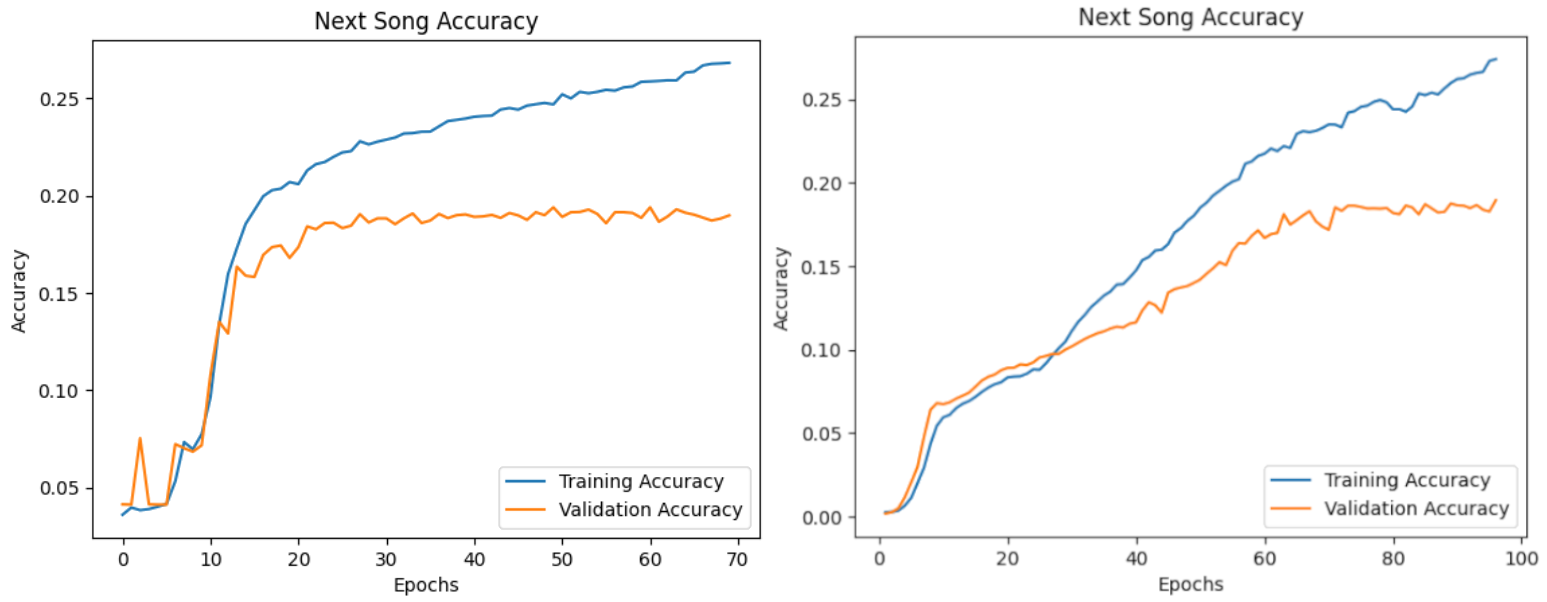
\includegraphics[width=\textwidth]{images/graph_attention_acc.png}
	\caption{Validation accuracies during training for the Bi-Directional LSTM model (Model 2; \emph{left}) and for the Self-Attention model (Model 3; \emph{right}).}
\end{figure}

\begin{table}
	\caption{Summary of Model Training Results}
	\label{results-table}
	\centering
	\begin{tabular}{lll}
		\toprule
		Model & Best Next-Song Validation Accuracy & Generated Sequence Quality \\
		\midrule
		2019 Model Recreation & $\sim$12.5\% & Not Attempted \\
		Model 1 & $\sim$18\% & Poor \\
		Model 2 & 19.5\% & Moderate \\
		Model 3 & 19.0\% & Moderate \\
		Model 4 & 16.8\% & Good \\
		\bottomrule
	\end{tabular}
\end{table}

All of the new models were able to outperform the recreated 2019 model in terms of next song accuracy, although the sequences that they generated were of varying degrees of quality. For example, Model 1 was able to predict a sequence of songs without repeats, but was not able to predict part-of-speech separators like 'set-1' or 'eos'. In contrast, Model 2 was able to predict part-of-speech separators but was unable to always do this in a way that made sense. It also missed many common sequential orderings of songs like 'The Horse' into 'Silent in the Morning'. Model 3 had better predictions for part-of-speech separators which were all sensical, although it repeated and alternated songs often. The band sometimes does this during shows so it is not an outlandish prediction, but Model 3 does this a little \emph{too} often to be considered a good prediction. Model 4 generated the best predictions with good placements for the part-of-speech separators and few repeated songs, despite it's lower next song accuracy compared to models 2 and 3. 

Another evaluation method extends beyond predicting the $n^{th}$ song and instead assesses the model's capability to predict the next $n$ songs, or its accuracy in predicting the next sequence. To do this, Models 2, 3, and 4 were fed a seed sequence of a few songs from the beginning of a longer test setlist. Then the results of the model predictions from the seed sequence were compared to the actual next songs \emph{irrespective of song order}. 

For each model, the setlist used for comparison was as follows with the first three songs used as the seed: 

\begin{center}
	['farmhouse', 'first-tube', 'twist', 'divided-sky', 'ginseng-sullivan', 'carini', 'whats-the-use', 'wildcard', 'set-2', 'down-with-disease', 'the-moma-dance', 'piper', 'fee', 'gotta-jibboo', 'saw-it-again', 'split-open-and-melt', 'cavern', 'david-bowie', 'set-e', 'the-squirming-coil', 'eos']
\end{center}

Table 2 shows the results of this exercise. Models 2, 3, and 4 were all able to achieve similar accuracies in this regard. They all correctly predicted part-of-speech separators which would be used, and were able to predict a few songs which would appear in the next setlist. 

\begin{table}
	\caption{Summary of Model Training Results}
	\label{generation-table}
	\centering
	\begin{tabular}{lll}
		\toprule
		Model & Common Songs (Original \& Prediction) & Accuracy \\
		\midrule
		Model 2 & ['set-2', 'down-with-disease', 'set-e', 'piper', 'eos', 'the-moma-dance'] & 33.33\% \\
		Model 3 & ['wildcard', 'set-2', 'set-e', 'david-bowie', 'cavern', 'eos'] & 33.33\% \\
		Model 4 & ['set-e', 'wildcard', 'piper', 'the-moma-dance', 'eos', 'set-2'] & 33.33\% \\
		\bottomrule
	\end{tabular}
\end{table}

\section{Discussion}

Considering the probability of random chance and given the small, diverse, and random nature of this "language" of song sequences, achieving above 16\% accuracy with multiple distinct model architectures shows these small language models are able to identify impactful features to a decent degree. Although we hoped to improve the accuracy beyond that obtained in the original 2019 experiment, we were unable to cross the 20\% next song accuracy mark. However, given we were unable to reproduce the original experiment to the same degree of accuracy as achieved previously, the results shown here significant. In particular, it is shown that Attention-based models are able to slightly outcompete the RNN LSTM model in terms of generative quality, and can be near peers in terms of next song accuracy. 

Further experimentation on this subject could expand upon this work in the following ways:
\begin{itemize}
	\item Giving the models additional context for songs, such as key, tempo, or lyric sentiment, could greatly increase the within setlist predictive capability by generating better song transitions.
	\item Giving the models additional context for shows, such as date, venue, or location, could also help to improve long-term temporal predictions. For example, 'Auld-Lang-Syne' is always and only ever performed on new year's eve. 
	\item Additional model architectures could be tried - in particular generative adversarial networks (GANs) and conditioned variational autoencoders (CVAE) models would likely excel in the generation part.
	\item Dynamic Temporal Graphs could be used to model changing probabilities over time, and modelling song sequences as random walks with the prior temporal information could be a promising avenue to generate new setlists and predict song sequences [8, 9]. 
	\item Audio signal sequencing to learn sentiments and transitional markers for songs could be another way to improve song to song prediction accuracy. 
	\item This approach could be extended to other artist's. Although Phish has a large catalog of music, The Grateful Dead in particular has a similarly sized catalog of music and tendencies which could be interesting to explore. 
\end{itemize} 

\section{Conclusion}

The greatest obstacle for small language models is the size of the training dataset and the underlying structure of the language phenomenon which is being modeled. Despite this, RNNs and Attention-based transformer models can learn the syntactical tendencies of small languages to a limited degree. Despite being unable to recreate a 2019 project which attempted to model the music of Phish in this way, this project was able to reconstruct LSTM models to accomplish the same task with similar levels of accuracy and employ new Attention-based models to exceed the generative abilities of the RNN models. Additional work in this field should strongly consider the addition of more contextual information in the form of song or show attributes, temporal graph models, or audio signal sequencing.

The code we used to acquire and process the dataset, train and evaluate our models is available at \url{https://github.iu.edu/rjdharmc/dlProject}.\footnote{Note that access to this codebase will require an active account on the IU Enterprise Github instance.}

\section*{References}

{
	\small
	
	
	[1] F. Tomasi, J. Cauteruccio, S. Kanoria, K. Ciosek, M. Rinaldi, and Z. Dai, “Automatic Music Playlist Generation via Simulation-based Reinforcement Learning,” Proceedings of the 29th ACM SIGKDD Conference on Knowledge Discovery and Data Mining. ACM, Aug. 04, 2023. doi: 10.1145/3580305.3599777. 
	
	[2] R. T. Irene, C. Borrelli, M. Zanoni, M. Buccoli, and A. Sarti, “Automatic playlist generation using Convolutional Neural Networks and Recurrent Neural Networks,” 2019 27th European Signal Processing Conference (EUSIPCO). IEEE, Sep. 2019. doi: 10.23919/eusipco.2019.8903002. 
	
	[3] K. Choi, G. Fazekas, and M. Sandler, “Towards Playlist Generation Algorithms Using RNNs Trained on Within-Track Transitions.” arXiv, 2016. doi: 10.48550/ARXIV.1606.02096. 
	
	[4] T. Mikolov, K. Chen, G. Corrado, and J. Dean, “Efficient Estimation of Word Representations in Vector Space.” arXiv, 2013. doi: 10.48550/ARXIV.1301.3781.
	
	[5] A. Vaswani, N. Shazeer, N. Parmar, J. Uszkoreit, L. Jones, A. N. Gomez, L. Kaiser, and I. Polosukhin, “Attention Is All You Need.” arXiv, 2017. doi: 10.48550/ARXIV.1706.03762.
	
	[6] A. Radford, J. Wu, R. Child, D. Luan, D. Amodei, and I. Sutskever. "Language models are unsupervised multitask learners". 2019.
	
	[7] A. Radford, K. Narasimhan, T. Salimans, and I. Sutskever. "Improving Language Understanding by Generative Pre-Training". 2017.
	
	[8] D. Gurevin, M. Shan, T. Geng, W. Jiang, C. Ding, and O. Khan, “Towards Real-Time Temporal Graph Learning.” arXiv, 2022. doi: 10.48550/ARXIV.2210.04114. 
	
	[9] Y. Shen, J. Chen, P.-S. Huang, Y. Guo, and J. Gao, “M-Walk: Learning to Walk over Graphs using Monte Carlo Tree Search.” arXiv, 2018. doi: 10.48550/ARXIV.1802.04394.
}

\end{document}